%% Le travail effectué [10-20 pages]
%% Vous devez montrer les points conceptuels et techniques importants :
%% Étude du cahier des charges
%% Propositions et critiques de solutions
%% Description complète de la solution choisie
%% Mise en oeuvre
%% Résultats obtenus (critique)

\section{Étude du cahier des charges}
\label{CDC}
\subsection{L’espace intranet \texttt{wordpress}}
Pour la première partie du stage concernant l’espace intranet, l’utilisation du \texttt{wordpress} et \texttt{GoogleDoc} fonctionne bien, le formulaire est généré automatiquement par \texttt{GoogleDoc} et les données sont envoyées vers le compte \texttt{Google} qui les a déjà enregistrées. Mais il y a quelques inconvénients supplémentaires à ceux présentés dans le sujet de stage si on utilise cette méthode:\\

\begin{itemize} 
\item Les données ne peuvent être visualisées qu'en format XSL dans un compte \texttt{GoogleDoc}
\item Il faut créer un compte Google public 
\item Le formulaire généré par \texttt{GoogleDoc} est trop simple, et n'a pas de fonctionnalités avancées \\
\end{itemize}

Donc il faut chercher une autre méthode pour présenter le formulaire et un moyen plus efficace pour exporter les données envoyées par les clients.  

\subsection{L’échange d’information avec FTP}

Pour la deuxième partie du stage concernant l’échange d’information et l'homogénéité des fichiers, le transfert des fichiers internes est supporté actuellement par un serveur FTP, mais toutes les opérations pour les fichiers doivent être faites manuellement, on a besoin d'ajouter une procédure de synchronisation des fichiers entre les machines locales et les machines à distances.\\

L'objectif est de metrre en place un système figuré ci-dessous: Les administrateurs ont les droits R\&W, c'est-à-dire lire et écrire des fichiers dans le serveur, les clients ont le droit W seulement, et s'ils veulent modifier les fichiers sur FTP, il faut envoyer un mail de notification aux administrateurs.\\

Les fichiers sont synchronisés entre un serveur local et le serveur FTP, les fichiers sur le serveur local sont synchronisés partiellement avec les ordinateurs des administrateurs.

\begin{figure}[!htbp]
  \centering
    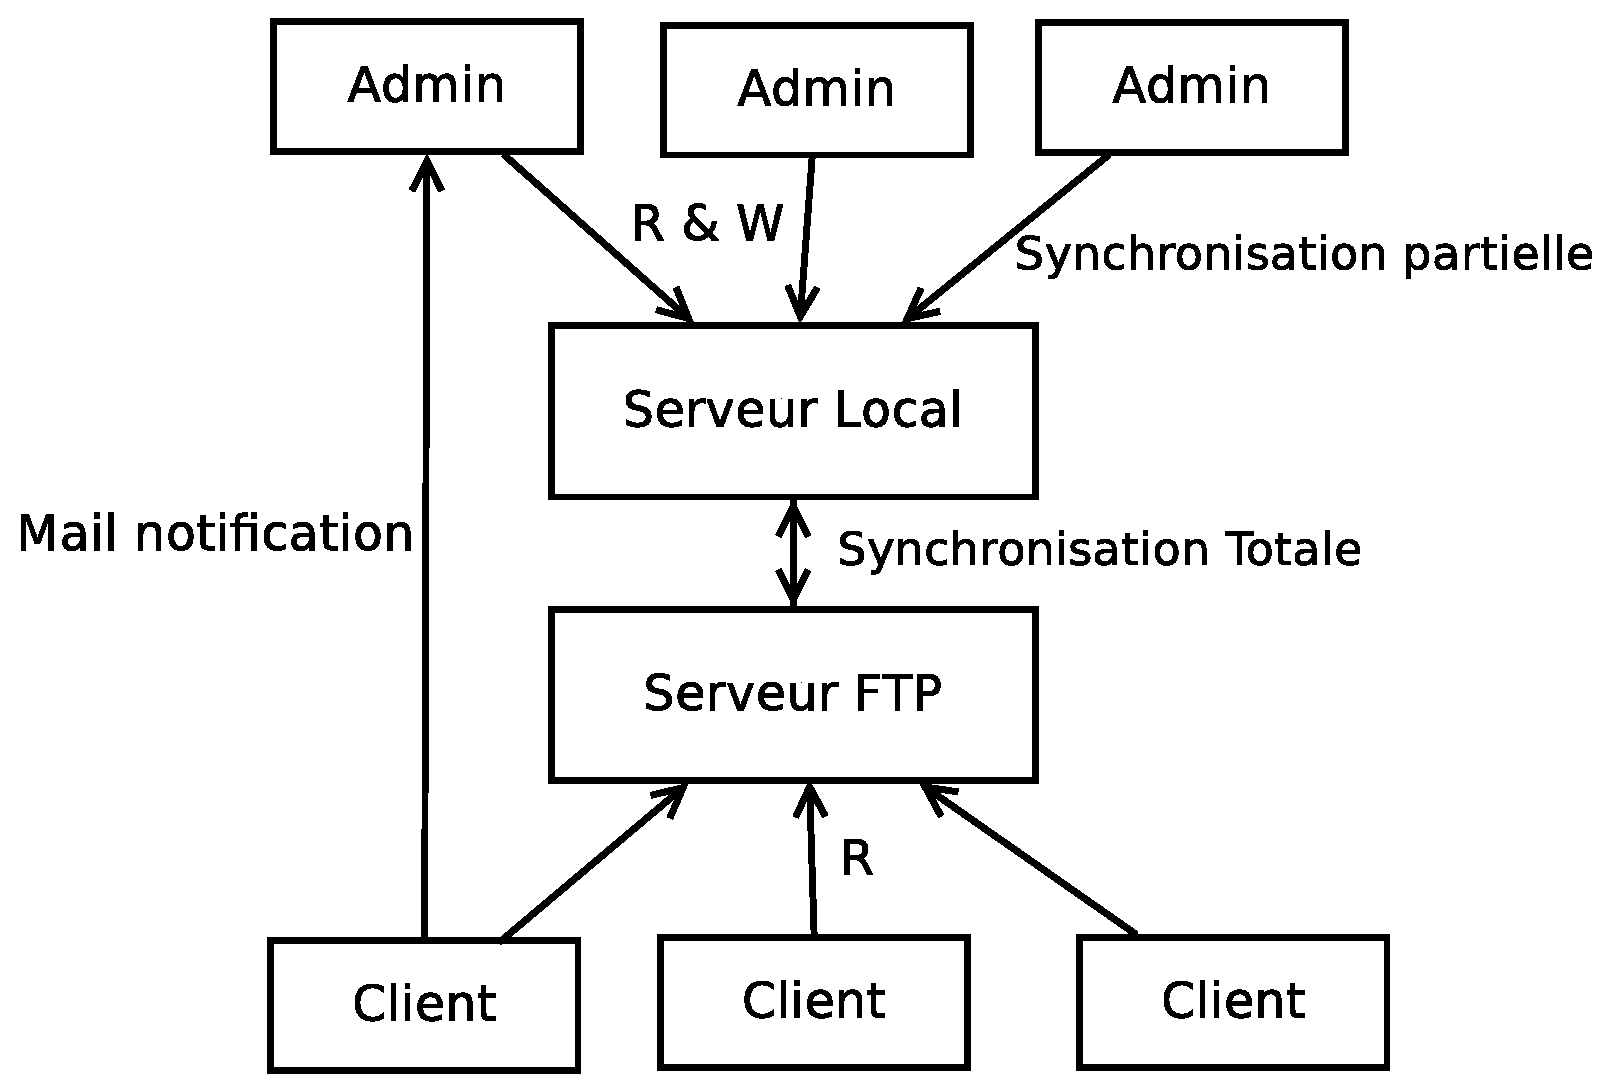
\includegraphics[scale=0.5]{images/FTP}
  \caption{L'objectif d'utilisation du FTP}
  %\label{fig:auth}
\end{figure} 
%%%%%%%%%%%%%%%%%%%%%%%%%%%%%%%%%%%%%%%%%%%%%%%%%%%%%%%%%%%%%%%%%%%%%%%%%%%%%%%%%%%%%%%%%%%%%%%%
\section{Propositions des solutions possibles}

  \subsection{L’espace intranet \texttt{wordpress}}
Pour l'espace intranet, je conseille de conserver le modèle wordpress mais de remplacer l'outil \texttt{GoogleDoc} par une extension wordpress qui s'appelle \texttt{WordPress Form Manager}, qui est destinée pour générer les formulaires professionnels.

     \subsubsection{Wordpress}


\begin{wrapfigure}[]{r}{70mm}
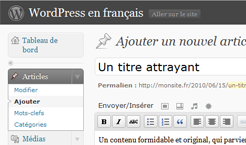
\includegraphics[scale=0.8]{images/wordpress.png}
\caption{Page d'adminisrtation de \texttt{wordpress}}
\end{wrapfigure}


WordPress est un système de gestion de contenu (CMS) qui permet de créer et gérer facilement l'ensemble d'un site web ou simplement un blog. Gratuit et libre, WordPress est personnalisable grâce à de nombreux thèmes et plugins(extensions).\\

En outre, il existe une solide communauté à travers le monde entier.\\

WordPress constitue le nec plus ultra en matière de plates-formes sémantiques de publication personnelle, alliant esthétique, standards du Web et ergonomie. Gratuit, WordPress n ’en est pas moins inestimable. Sous licence GPLv2+, cet outil est libre de droits.\\

Plus simplement, WordPress est ce qu’il nous faut si on veut avancer au moyen d’un système de gestion de contenu.\\





    \subsubsection{Les plugins du \texttt{wordpress}}
Les plugins permettent d'étendre les fonctionnalités de wordpress. Les plugins du wordPress peut s'étendre de faire presque tout ce qu'on peut imaginer, ils sont généralement crées par tout le monde, gratuits, et open-source. Dans notre site, on utilise quelques plugins:\\

\begin{itemize}
\item WordPress Form Manager
\item Database Browser
\item Configure SMTP
\item Code Insert Manager
\item etc.
\end{itemize}

    \paragraph{WordPress Form Manager}

WordPress Form Manager est un gestionnaire de formulaires qui stocke dans une table les informations fournies par les utilisateurs. Le plugin permet la gestion de fichiers joints et de captchas. La création de formulaires est très intuitive et une documentation très riche existe. Dans les plus: un affichage de formulaires interactif. Par exemple, on peut demander à afficher un champ texte uniquement lorsque l’utilisateur aura coché un certain bouton plus haut dans le formulaire. C’est une fonction impressionnante qui permet de complexifier sans lourdeur un formulaire. Dans les moins: la gestion de présentation des mails envoyés est vraiment très compliquée. Par défaut, les contenus des champs sont présentés sous forme de liste.\\
  
Form Manager est un outil pour créer des formulaires pour collecter et télécharger des données de visiteurs du site WordPress. Les formulaires sont ajoutés à des articles ou des pages en utilisant un shortcode simple, ou peut être ajouté au thème avec une API simple.\\

\begin{wrapfigure}[]{r}{80mm}
\centering
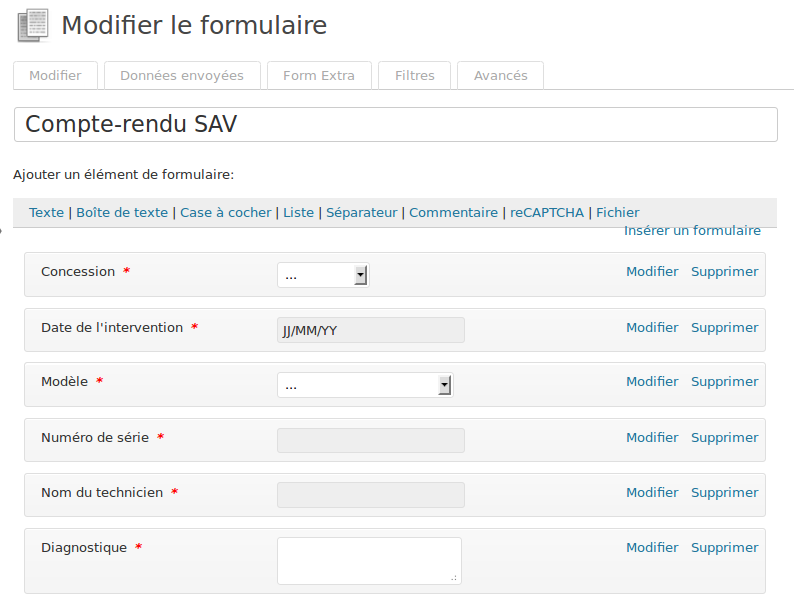
\includegraphics[scale=0.25]{images/formManager}
\caption{Page d'adminisrtation de plugin \texttt{Form Manager}}
\end{wrapfigure}

Les fonctionnalités:
\begin{itemize}
\item validation
\item champs requis
\item remerciements personnalisés
\item notifications par email
\item templates d'affichage des formulaires\\
\end{itemize}

Types de champs supportés:
\begin{itemize}
\item texte
\item zone de texte
\item liste déroulante
\item bouton radio
\item cases à cocher
\item sélection multiple
\item téléchargement
\item reCAPTCHA
\end{itemize}

    \paragraph{Database Browser}
Database Browser est un gestionnaire de base de données qui permet de connecter à notre serveur SQL, Oracle ou ODBC, d'en modifier les données, de les tester avec des scripts SQL mais également d'exporter et d'imprimer les données. L'application supporte un nombre illimité de connexions et permet de naviguer dans les tables rapidement et facilement. Un outil de recherche, un historique, un module d'exécution des fichiers LOG et d'autres options sont également disponibles.

  \subsection{L’échange d’information avec FTP}
  \label{infoFTP}
Avec le cahier de charge ci-dessus, je propose de concevoir une application Web qui a pour objectif de réaliser les opérations concernant le FTP, par exemple:\\

\begin{itemize}
\item On peut se connecter avec deux comptes différents, un compte administrateur et un compte utilisateur
\item Tous les utilisateurs peuvent visualiser les données dans le serveur FTP
\item Il y a une liste de demandes de changement des fichiers donnée par le client, si on se connecte avec le compte administrateur, on peut les autoriser ou les refuser\\
\end{itemize}

Pour la procédure de synchronisation, il y en a pas mal de logiciels qui existent déjà.

%%%%%%%%%%%%%%%%%%%%%%%%%%%%%%%%%%%%%%%%%%%%%%%%%%%%%%%%%%%%%%%%%%%%%%%%%%%%%%%%%%%%%%%%%%%%%%%%
\section{Mise en oeuvre}
  \subsection{Phrase de préparation}
Les exigences minimales pour exécuter WordPress sont:

\begin{itemize}
\item PHP version 5.2.4 
\item MySQL version 5.0 \\
\end{itemize}

Dans ce cas, on a besoin:
\begin{itemize}
\item de l’accès d'un serveur FTP
\item d'un logiciel puissant permettant de manipuler les fichiers sur le serveur FTP 
\item d'un système d'exploitation de type linux
\item de l'environnement PHP
\item de l'environnement base de donnée MySQL
\item de la ré-installation du \texttt{wordpress}
\item d'un logiciel pour manipuler la base de donnée (\texttt{phpMyAdmin} par exemple)
\end{itemize}

     \subsubsection{connecter au serveur FTP} 
Le DSI m'a donné un compte pour accéder au serveur FTP de la société, qui a les droits d'écrire et de modifier les fichiers.\\

Pour la manipulation des fichiers dans le FTP, il a recommandé le logiciel \texttt{FileZilla}.\\

FileZilla est un client FTP. Un logiciel libre qui permet de charger ou télécharger les fichiers sur un serveur. Il possède une interface utilisateur graphique intuitive. On choisie ce logiciel pour les raisons suivants:\\

\begin{itemize}
\item logiciel Open-source
\item Rapide et fiable, facile à utiliser
\item Multi-plateforme. Fonctionne sur Windows, Linux, BSD, Mac OS X et plus. C'est importante parce que les personnes dans l'équipe utilisent les différents types de OS.
\item Disponible dans de nombreuses langues, car les clients viennent des differents pays
\end{itemize}


     \subsubsection{Installation l'OS Ubuntu}
À l'INSA, on utilise beaucoup le système d'exploitation de type linux, Ubuntu par exemple.
Ubuntu est un système d’exploitation libre commandité par la société Canonical et c'est une marque déposée par cette même société.\\

Fondé sur la distribution Linux Debian et utilisant le bureau Unity, Ubuntu se veut « convivial, intuitif et sûr ». Il est constitué de logiciels libres, est disponible gratuitement y compris pour les entreprises, et bénéficie d'une nouvelle version tous les six mois.\\

Avec une utilisation globale estimée à plus de 25 millions d'utilisateurs, il est principalement conçu pour une utilisation sur des ordinateurs personnels (portables et fixes), bien que d'autres versions consacrées aux netbooks et aux serveurs existent aussi. \\

     \subsubsection{Installation d'environnement PHP}
Pour faire fonctionner \texttt{wordpress}, il faut un environnement PHP sur le serveur.
Je l'ai installé suivant les instructions du cours Technologie Web encadré par M.Alexandre Pauchet:\\
 
\begin{itemize}
\item Récupérer des sources dans \url{http://www.apache.org} et \url{http://www.php.net} et déposer les 2 archives dans \texttt{<chemin>/srcweb}
\item Décompression des sources
\item Configuration de la compilation
\item Compilation
\item Test d'Apache et du module PHP dans Apache
\end{itemize}

     \subsubsection{Installation de la base de donnée}
     \label{database}
Si on utilise le CMS \texttt{wordpress}, il faut une base de données associée à ce site, pour ce faire, j'ai installé la base de données avec \texttt{MySQL}. On peut créer un tableau facilement avec quelques lignes de commande.

     \subsubsection{Mise en place de Wordpress}
\begin{itemize}
\item[Étape 1:]Téléchargez et décompressez WordPress.
\item[Étape 2:]Créez une base de données pour WordPress sur le serveur Web(Voir \ref{database}), de sorte que MySQL ait tous les privilèges en accès et en modification.
\item[Étape 3:]Ouvrez le fichier \texttt{wp-config.php} dans l'éditeur de texte et complétez les informations de la base de données (et le langage utilisé par le blog si nécessaire).
\item[Étape 4:]Déposez les fichiers de WordPress à l'emplacement désiré sur votre serveur Web :
\item[Étape 5:]Comme on a téléchargé la version anglaise de WordPress, vous devez copier les fichiers de traduction fr\_FR.mo et continents-cities-fr\_FR.mo (correspondants à la version de WordPress installée) dans le sous-dossier \texttt{wp-content/languages}. Ensuite, modifiez le fichier \texttt{wp-config.php} pour avoir define ('WPLANG', 'fr\_FR')
\item[Étape 6:]Lancer le script d'installation de WordPress en ouvrant \texttt{wp-admin/install.php} dans votre navigateur Web préféré.
\end{itemize}    
 
     \subsubsection{Clés secrètes pour la base de données}    
Une clé secrète qui rend le site plus difficile à pirater et plus difficile à casser en ajoutant des éléments aléatoires pour le mot de passe.\\

En termes simples, une clé secrète est un mot de passe avec des éléments qui font qu'il est plus difficile de générer suffisamment d'options pour percer les barrières de sécurité. Un mot de passe comme "mot de passe" ou "test" est simple et se brisent facilement. Une aléatoire, imprévisible mot de passe tels que "88a7da62429ba6ad3cb3c76a09641fc" prend des années à venir avec la bonne combinaison.\\

Un exemple d'utilisation des clés secrètes:\footnote{extrait du tutoriel \texttt{Wordpress}}
\begin{verbatim}
define('AUTH_KEY',         't`DK%X:>xy|e-Z(BXb/f(Ur`8#~UzUQG-^_C');
define('SECURE_AUTH_KEY',  'D&ovlU#|CvJ##uNq}bel+^MFtT&.b9{UvR]g');
define('LOGGED_IN_KEY',    'MGKi8Br(&{H*~&0s;{k0<S(O:+f#WM+q|npJ');
define('NONCE_KEY',        'FIsAsXJKL5ZlQo)iD-pt??eUbdc{_Cn<4!d~');
define('AUTH_SALT',        '7T-!^i!0,w)L#JK@pc2{8XE[DenYI^BVf{L:');
define('SECURE_AUTH_SALT', 'I6`V|mDZq21-J|ihb u^q0F }F_NUcy`l,=o');
define('LOGGED_IN_SALT',   'w<$4c$Hmd%/*]`Oom>(hdXW|0M=X={we6;Mp');
define('NONCE_SALT',       'a|#h{c5|P &xWs4IZ20c2&%4!c(/uG}W:mAv');
\end{verbatim}



  \subsection{Mise en place du formulaire}

\begin{wrapfigure}[]{r}{80mm}
\centering
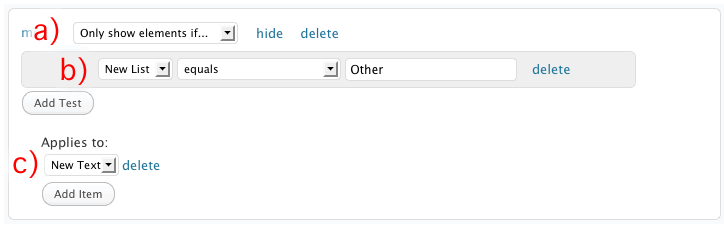
\includegraphics[scale=0.3]{images/form}
\caption{Un filtre du formulaire réalisé en \texttt{AJAX}}
\end{wrapfigure}

J'ai établi les formulaires en fonction des exigences des fournisseurs du Windeo Green futur, 
l’objectif des formulaires est de collecter les informations des différents turbines, mais chaque 
turbine a un type d'informations différent, donc il faut résumer les différents types de turbines 
et les mettre dans un seul formulaire.\\

Selon le type de turbine choisi, les lignes de formulaire apparaissent en fonction du choix de la turbine, pour ce faire, j'ai essayé de le faire avec AJAX, 
mais je n'y suis pas arrivé (explication en \ref{code}), donc on a cherché un autre plugin qui peut ajouter un filtre dans le formulaire comme figuré à droite. 

  \subsection{Mise en place d'une fonction d'authentification}

D'après la demande des personnes de la centrale d'achat, il faut ajouter une fonction d'authentification sur le wordpress, c'est-à-dire un mot de passe requis pour accéder aux pages du site. Mais malheureusement, le wordpress ne supporte pas cette fonctionnalité par défaut, donc il faut l'ajouter à la main.\\

D'abord, j'ai ajouté un fichier \texttt{login.php} dans le répertoire principal du site, qui est un script d'affichage, pour lire le mot de passe donné par l'utilisateur.\\

J'ai ensuite ajouté une partie de code PHP (Voir dans Annexe) dans le fichier \texttt{header.php}, qui utilise le concept \texttt{SESSION} dans PHP.\\

Les résultats sont figurés ci-dessous:\\

\begin{center}
\begin{tabular}{c c}
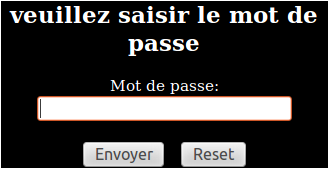
\includegraphics[scale=0.7]{images/auth1} & 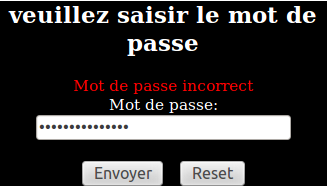
\includegraphics[scale=0.64]{images/auth2} \\
Page d'authentification & Page d'authentification en cas d'échec
\end{tabular}
\end{center}
%%%%%%%%%%%%%%%%%%%%%%%%%%%%%%%%%%%%%%%%%%%%%%%%%%%%%%%%%%%%%%%%%%%%%%%%%%%%%%%%%%%%%%%%%%%%%%%%
\section{Problèmes rencontrés}

\subsection{Exporter les données de wordpress}
\label{donnee}
Si on veut exporter les données du formulaire en format \texttt{.csv} avec le plugin \texttt{Database browser}, il apparaît un avertissement listé ci-dessous:\\
 
\begin{verbatim}
Warning: Cannot modify header information - 
headers already sent in /var/www/vhosts/windeo-planet.com/httpdocs/www/
wordpress/wp-content/plugins/wordpress-form-manager/getcsv.php on line 36

Warning: Cannot modify header information - 
headers already sent in /var/www/vhosts/windeo-planet.com/httpdocs/www/
wordpress/wp-content/plugins/wordpress-form-manager/getcsv.php on line 37

Warning: Cannot modify header information - 
headers already sent in /var/www/vhosts/windeo-planet.com/httpdocs/www/
wordpress/wp-content/plugins/wordpress-form-manager/getcsv.php on line 38

Warning: Cannot modify header information - 
headers already sent in /var/www/vhosts/windeo-planet.com/httpdocs/www/
wordpress/wp-content/plugins/wordpress-form-manager/getcsv.php on line 39
\end{verbatim}

qui concerne cette partie(lignes 36-39) du fichier \texttt{getcsv.php}:
\begin{verbatim}
header("Content-type: application/csv");
header("Content-Disposition: attachment; 
        filename=\"".$formInfo['title'].".csv\"");
header("Pragma: no-cache");
header("Expires: 0");
\end{verbatim}

Après la recherche sur Internet, cela est souvent dû à des lignes blanches ou espaces au début d'un fichier \texttt{.php}, ceux-ci doivent impérativement commencer par \texttt{<?php} et rien d'autre.
Après la vérification des fichiers concernés, je ne vois aucune ligne blanche ou espace avant \texttt{<?php}. Par ailleurs,  
dans wordpress, on ne peut pas toucher les fichiers générés (explication dans \ref{code}). Je suppose alors c'est peut-être à cause d'un conflit des plugins, mais je ne peux pas désactiver les autres plugins, ni faire de modifications, 
donc je propose deux solutions possibles:\\

\begin{itemize}
\item Désactiver l'avertissement du PHP
\item Chercher une autre méthode pour exporter les données \\
\end{itemize}

Finalement, j'ai choisi la mise en place de l'outil \texttt{phpMyAdmin} pour faire la gestion de la base de données:\\

\begin{wrapfigure}[]{r}{95mm}
\centering
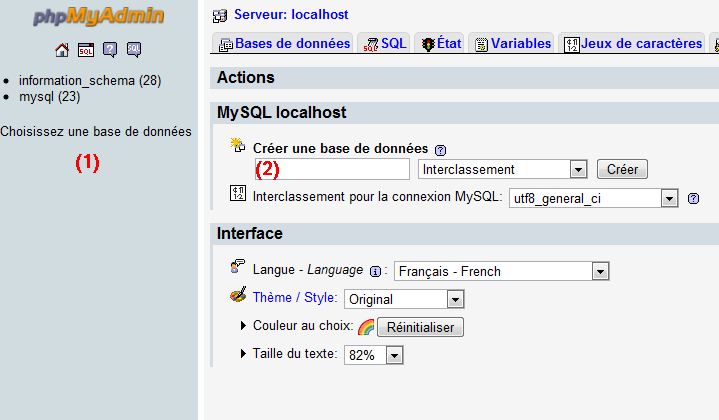
\includegraphics[scale=0.4]{images/phpmyadmin}
\caption{Capture d'écran \texttt{PhpMyAdmin}}
\end{wrapfigure}

phpMyAdmin (PMA) est une application Web de gestion pour les systèmes de gestion de base de données MySQL réalisée en PHP et distribuée sous licence GNU GPL.\\

Il s'agit de l'une des plus célèbres interfaces pour gérer une base de données MySQL sur un serveur PHP. De nombreux hébergeurs, qu'ils soient gratuits ou payants, le proposent ce qui permet à l'utilisateur de ne pas avoir à l'installer.\\

\subsection{Personnalisation du wordpress}
\label{code}
J'ai proposé de faire la personnalisation du \texttt{wordpress}, par exemple, d'ajouter les codes PHP dans une page qui existe déjà, faire le changement de mise en pages du formulaire, etc. Car la fonctionnalité du \texttt{wordpress} n'est pas suffisante, mais malheureusement ce n'est pas possible à ce moment-là. \\

En effet, on voulait bien ajouter une fonction \texttt{AJAX} pour faire un formulaire dynamique, mais je n'ai pas trouvé le fichier \texttt{.php} concernant ce formulaire. Après l'étude du wordpress plus profondément, j'ai trouvé le mécanisme de ce CSM: Il n'existe pas de fichiers réels pour chaque page, mais ils sont générés par les modèles définis par les fichiers \texttt{.php} du wordpress et par la base de données. Par exemple, si on veut faire l'affichage des données en format \texttt{csv} (présenté dans \ref{donnee}), le wordpress appelle le fichier \texttt{getcsv.php} dans dossier du plugin et les données stockées dans la base de donnée.\\

De cette façon, on ne peut pas faire la personnalisation des pages, sauf si on change les codes sources du plugin, ou si on remplace les plugins par un autre plugin. 

\subsection{Notifications par mail}

On a besoin d'envoyer un mail si un formulaire est rempli, mais si on fait un test, il y a toujours une erreur listée ci-dessous:

\begin{verbatim}
An error was encountered while trying to send the test e-mail.
SMTP Error: Could not connect to SMTP host.
\end{verbatim}

J'ai vérifié que les configurations de boîte mail et les portes des SMTP étaient correctes, mais l'ordinateur ne peut toujours pas se connecter au serveur SMTP. Après beaucoup de recherche sur Internet, j'ai vu une autre raison éventuelle: le serveur a interdit la fonction \texttt{fsockopen()} qui concerne la fonctionnalité de mail, on peut le remplacer par \texttt{pfsockopen()}, mais malheureusement, après la changement, ça ne fonctionnait toujours pas.\\

J'ai pensé ensuite que cela était peut-être dû aux configurations du serveur du site, donc j'ai envoyé un mail à la DSI pour demander de vérifier les configurations du SMTP sur le serveur, et la DSI m'a repondu que les portes de SMTP étaient fermées par défaut dans le serveur, après ce changement, cela a parfaitement fonctionné.

%%%%%%%%%%%%%%%%%%%%%%%%%%%%%%%%%%%%%%%%%%%%%%%%%%%%%%%%%%%%%%%%%%%%%%%%%%%%%%%%%%%%%%%%%%%%%%%%
\section{Résultats obtenus}
Enfin, j'ai mis en place 4 formulaires pour la société Windeo Green Futur:\\

\begin{itemize}
\item Formulaire d’installation
\item Formulaire maintenance ordinaire
\item Formulaire SAV
\item Formulaire type ARE\\
\end{itemize} 

C'est un exemple des formulaires qu'on a établi durant mon stage:

\begin{figure}[!htbp]
  \centering
    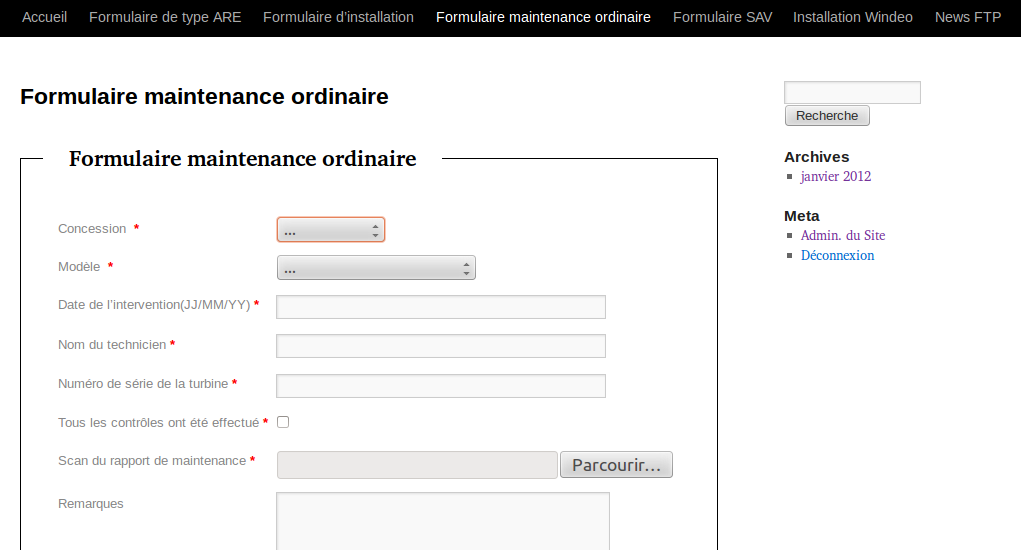
\includegraphics[width=\textwidth]{images/resultat}
  \caption{Capture d'écran du formulaire maintenance ordinaire}
  %\label{fig:auth}
\end{figure}

\newpage

Pour la deuxième partie du stage, on n'a pas eu assez de temps pour concevoir l'application Web décrite dans le Cahier des charges, donc j'ai conseillé d'utiliser un logiciel existant qui s'appelle GoodSync et qui a les fonctionnalités suffisantes pour les manipulations des fichiers FTP.\\

GoodSync est un logiciel de synchronisation de fichiers et de sauvegarde de fichiers qui opère automatiquement les syncs entre PC de bureau, portables et disques externes.\\

\begin{figure}[!htbp]
\centering
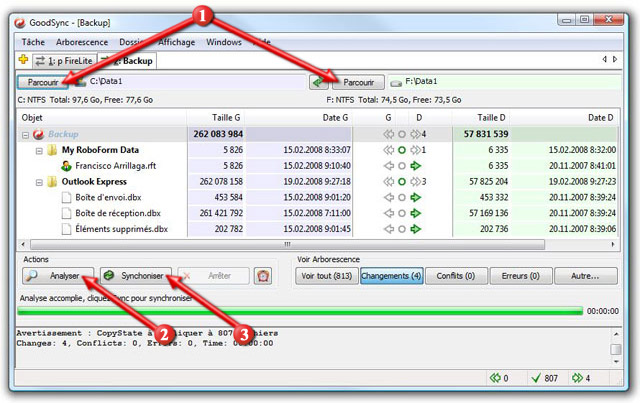
\includegraphics[scale=0.6]{images/Goodsync}
\caption{Logiciel \texttt{GoodSync}}
\end{figure}





